\begin{figure}[h!]
	\centering
	\begin{minipage}{.50\textwidth}
		\centering
		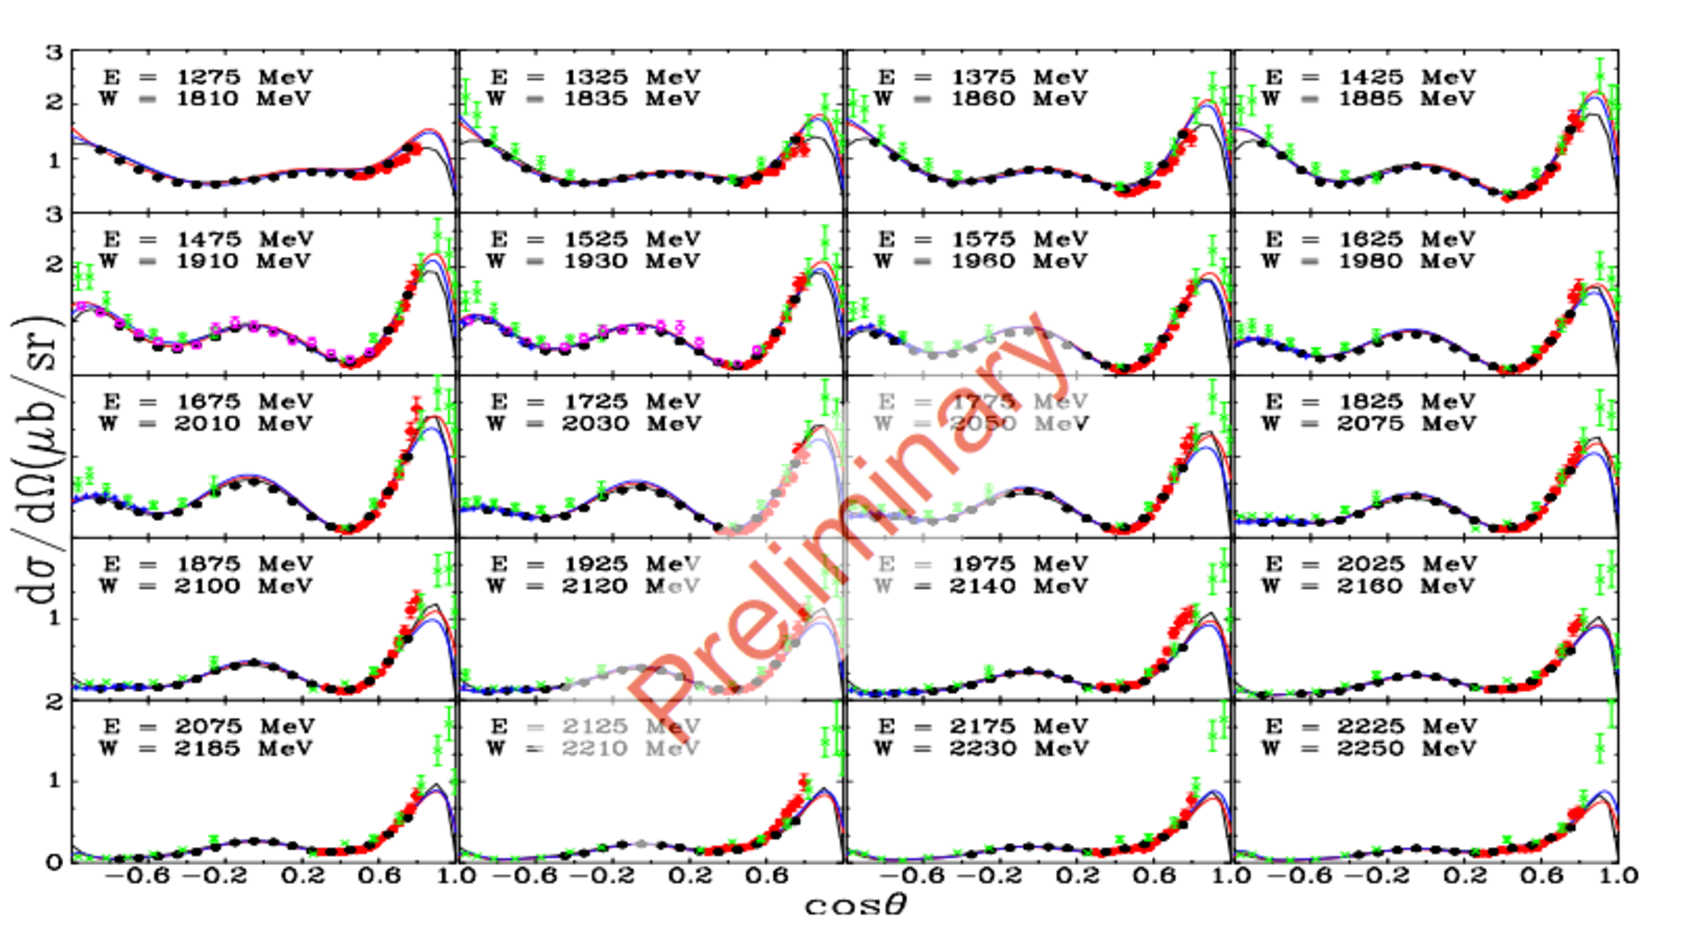
\includegraphics[width=225 pt, height = 160 pt]{figures/pi0_xsectionI.pdf}
		\caption{}{}
		\label{fig:pi0I}
	\end{minipage}%
	\centering
	\begin{minipage}{.50\textwidth}
		\centering
		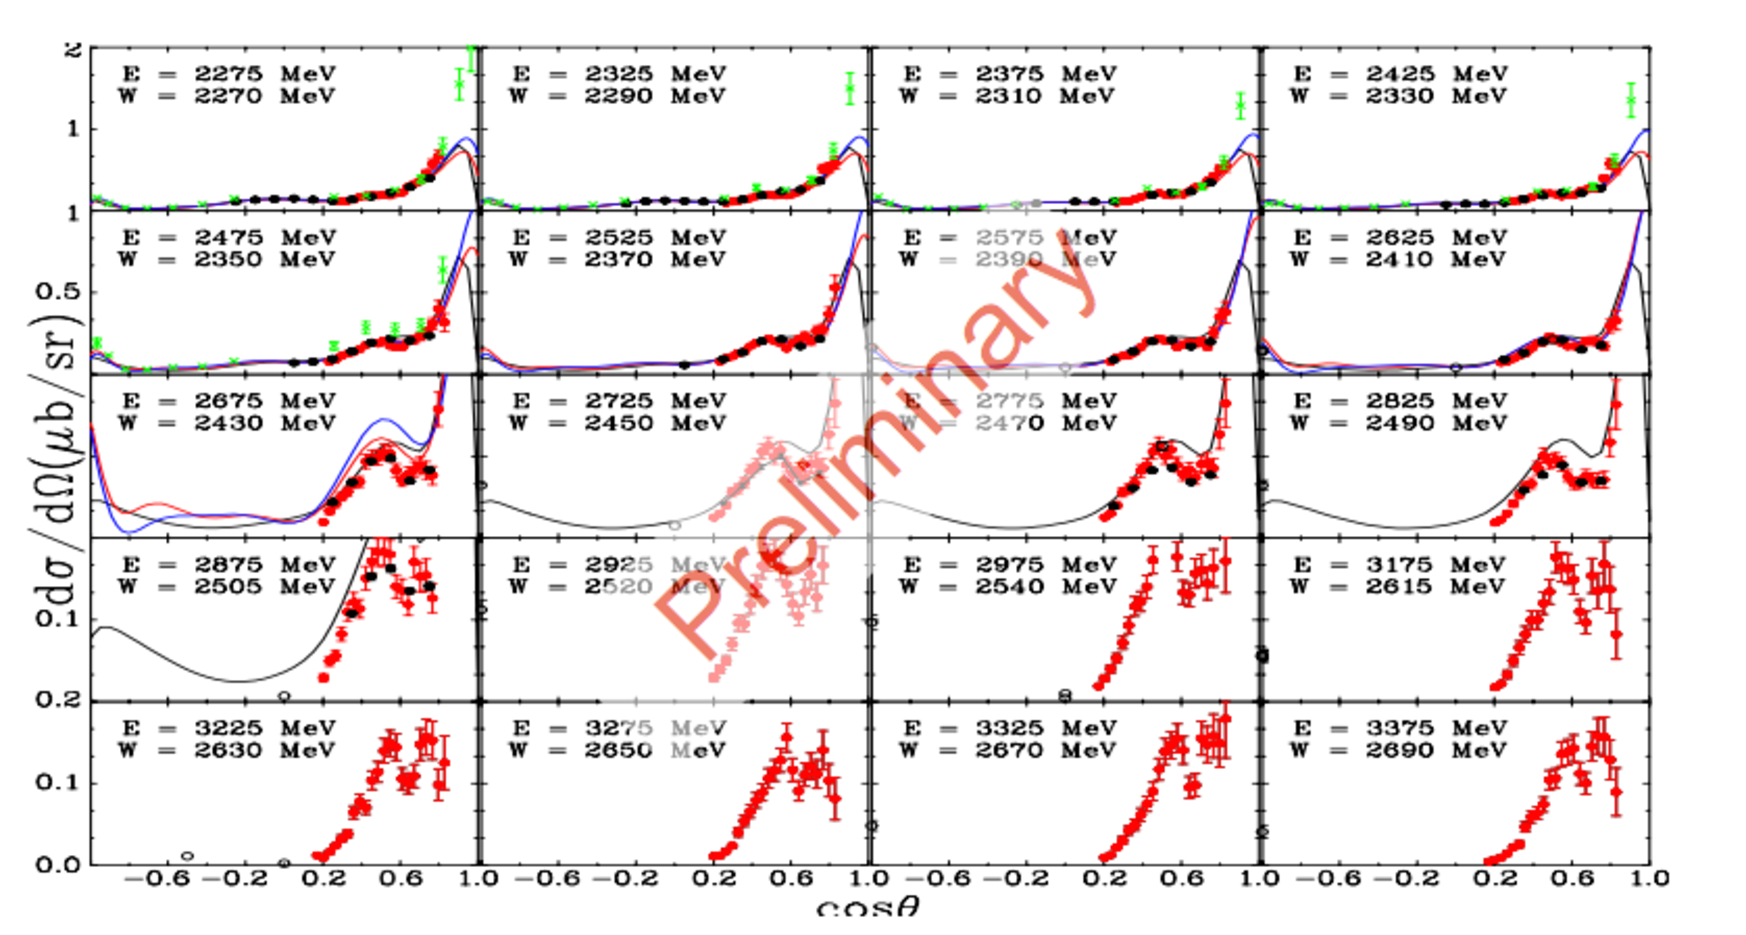
\includegraphics[width=225 pt, height = 160 pt]{figures/pi0_xsectionII.pdf}
		%\caption{figure in here}{box diagram}
		\caption{(Color online)The $\pi^0$ proton photoproduction cross section, $(d\sigma/d\Omega)$, at $E_{\gamma}$ = 1.275 -- 2.225~GeV versus $\cos\theta$ where $\theta$ is the pion center-of-mass production angle. Photon energy is indicated by $E$, while the center-of-mass total energy is indicated by $W$. Red solid (blue solid) lines show the SAID KU14 (DU13~\protect\cite{Dugger13}) calculations. Black solid lines give the BG2011-02 BnGa~\protect\cite{BonnGat}) predictions. Experimental data are from the current measurement (red filled circles), CLAS~\protect\cite{Dugger07} (black filled circles), GRAAL~\protect\cite{Graal} (magenta open circles), LEPS~\protect\cite{LEPS} (blue plus), CB-ELSA~\protect\cite{ELSA05}~\cite{ELSA11} (green crosses) and previous bremsstrahlung measurements~\protect\cite{brem} (black open circles). Plotted uncertainties are statistical. The plotted points from previously published experimental data are those data points within $\pm$3~MeV of the photon energy indicated on each panel.}{}
		\label{fig:pi0II}
	\end{minipage}
\end{figure}


\begin{figure}[h!]
	\centering
	\begin{minipage}{.50\textwidth}
		\centering
		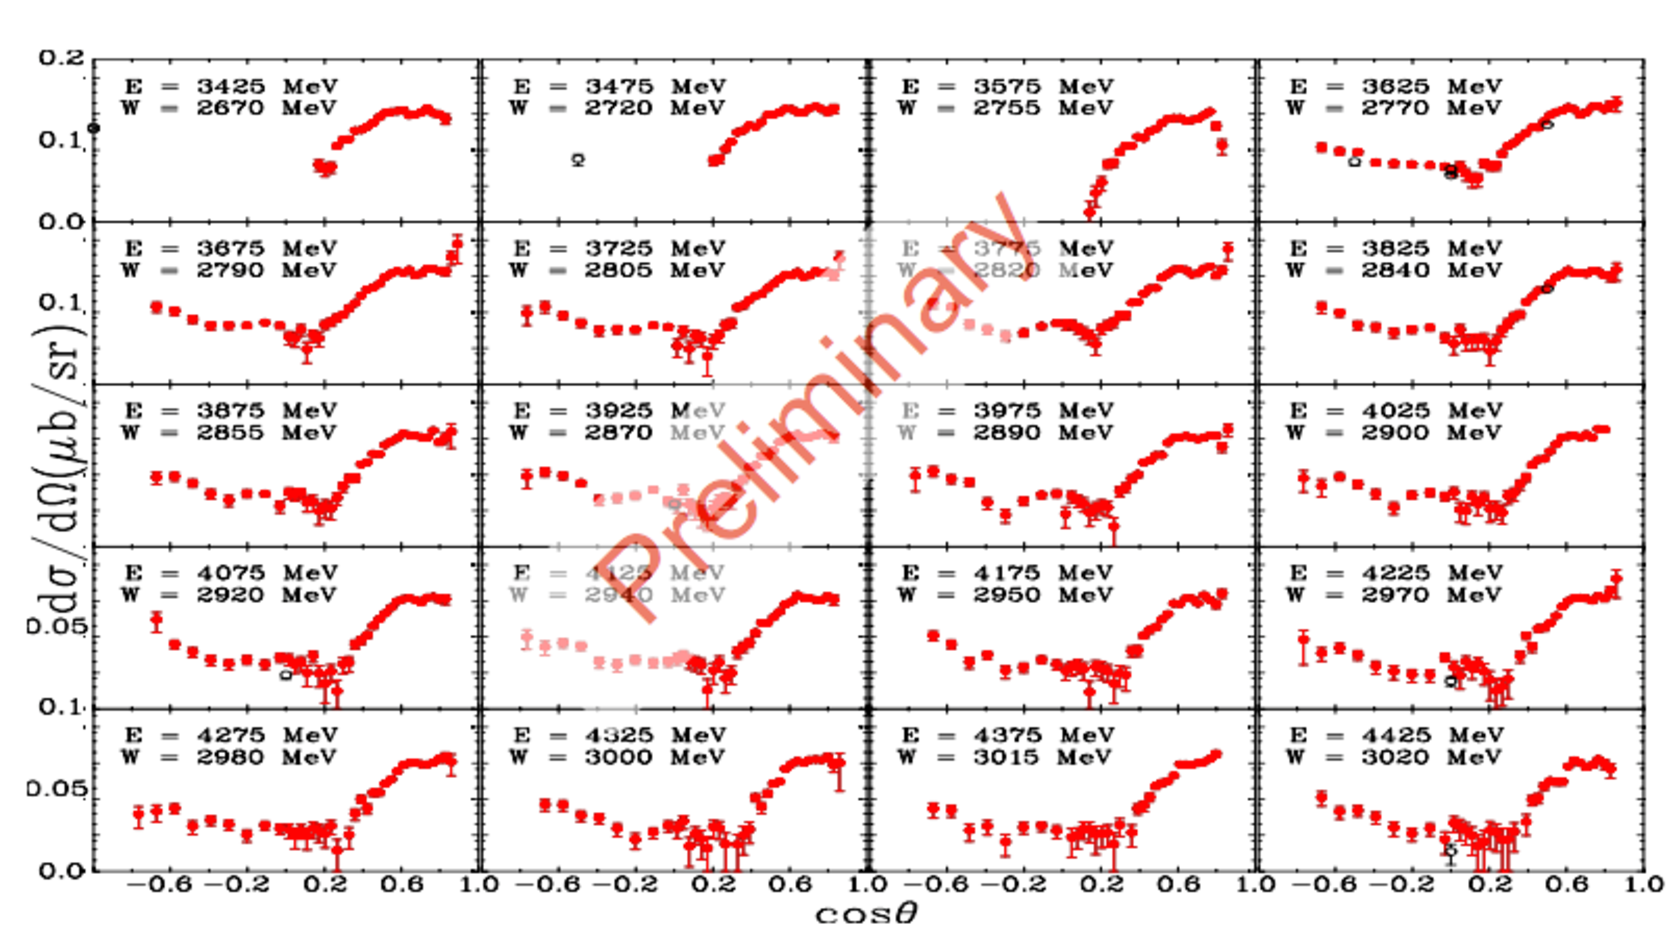
\includegraphics[width=225 pt, height = 160 pt]{figures/pi0_xsectionIII.pdf}
		\caption{}{}
		\label{fig:pi0III}
	\end{minipage}%
	\centering
	\begin{minipage}{.50\textwidth}
		\centering
		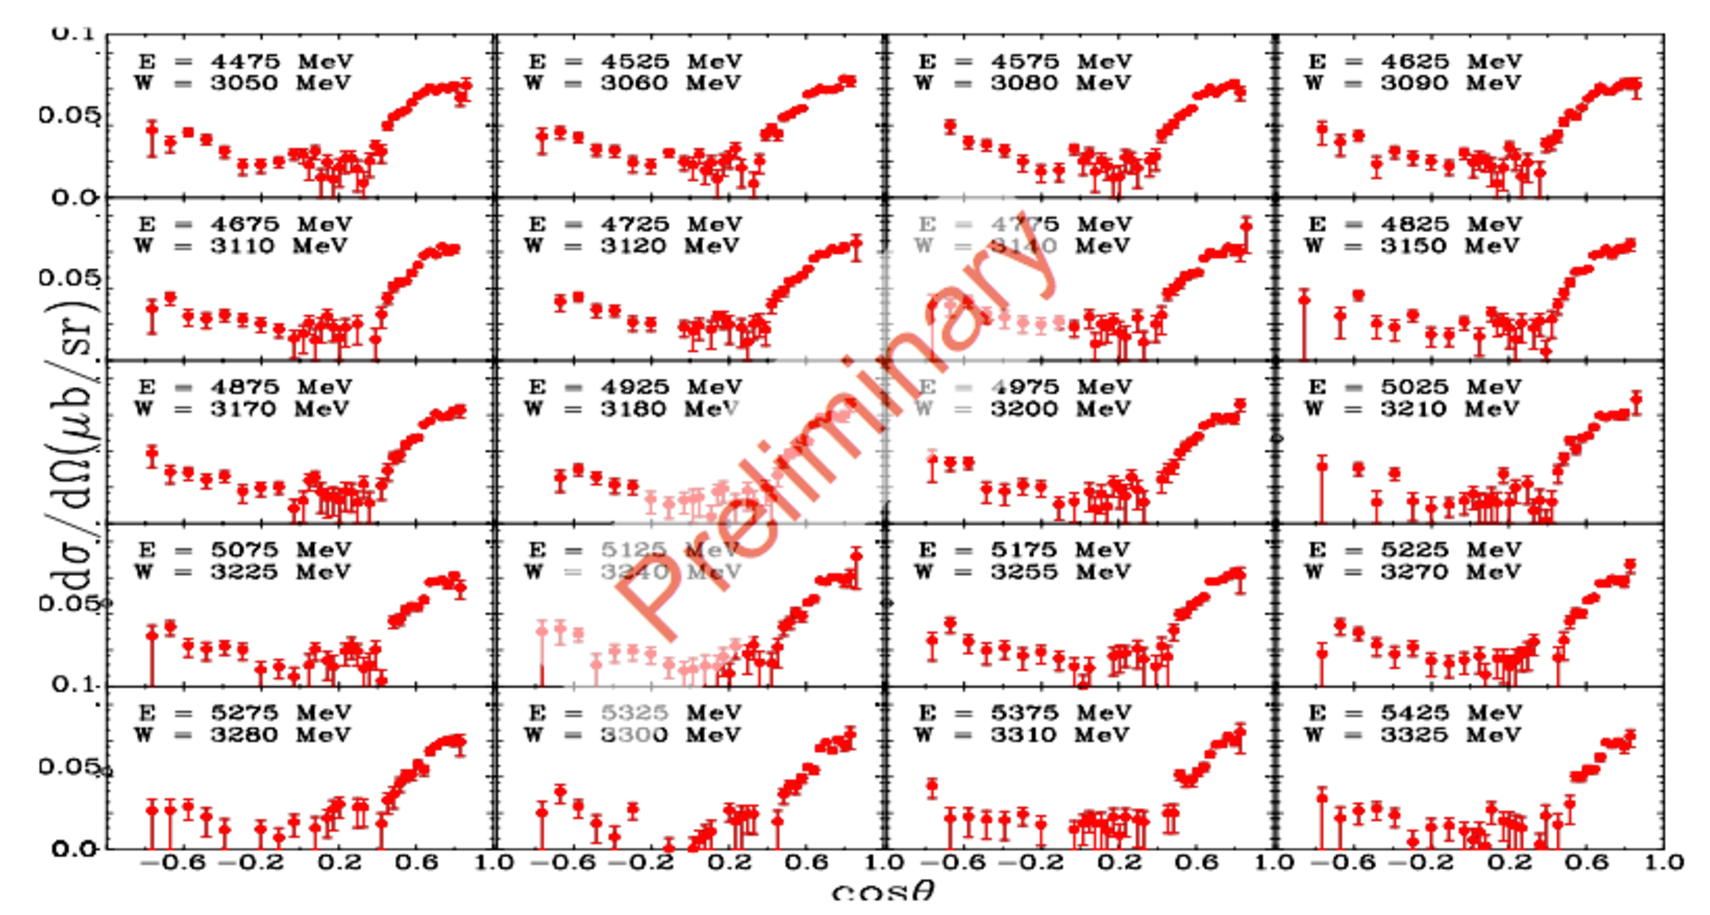
\includegraphics[width=225 pt, height = 155 pt]{figures/pi0_xsectionIV.pdf}
		%\caption{figure in here}{box diagram}
		\caption{(Color online)The $\pi^0$ proton photoproduction cross section at $E_{\gamma}$ = 3.425 -- 4.425~GeV(left):$E_{\gamma}$ = 4.475 -- 5.425~GeV(right) versus cosine of the pion center-of-mass production angle. Notation as in Fig.~\protect\ref{fig:pi0II}.}{}
		\label{fig:pi0IV}
	\end{minipage}
\end{figure}

\begin{figure}[h]
	\centerline{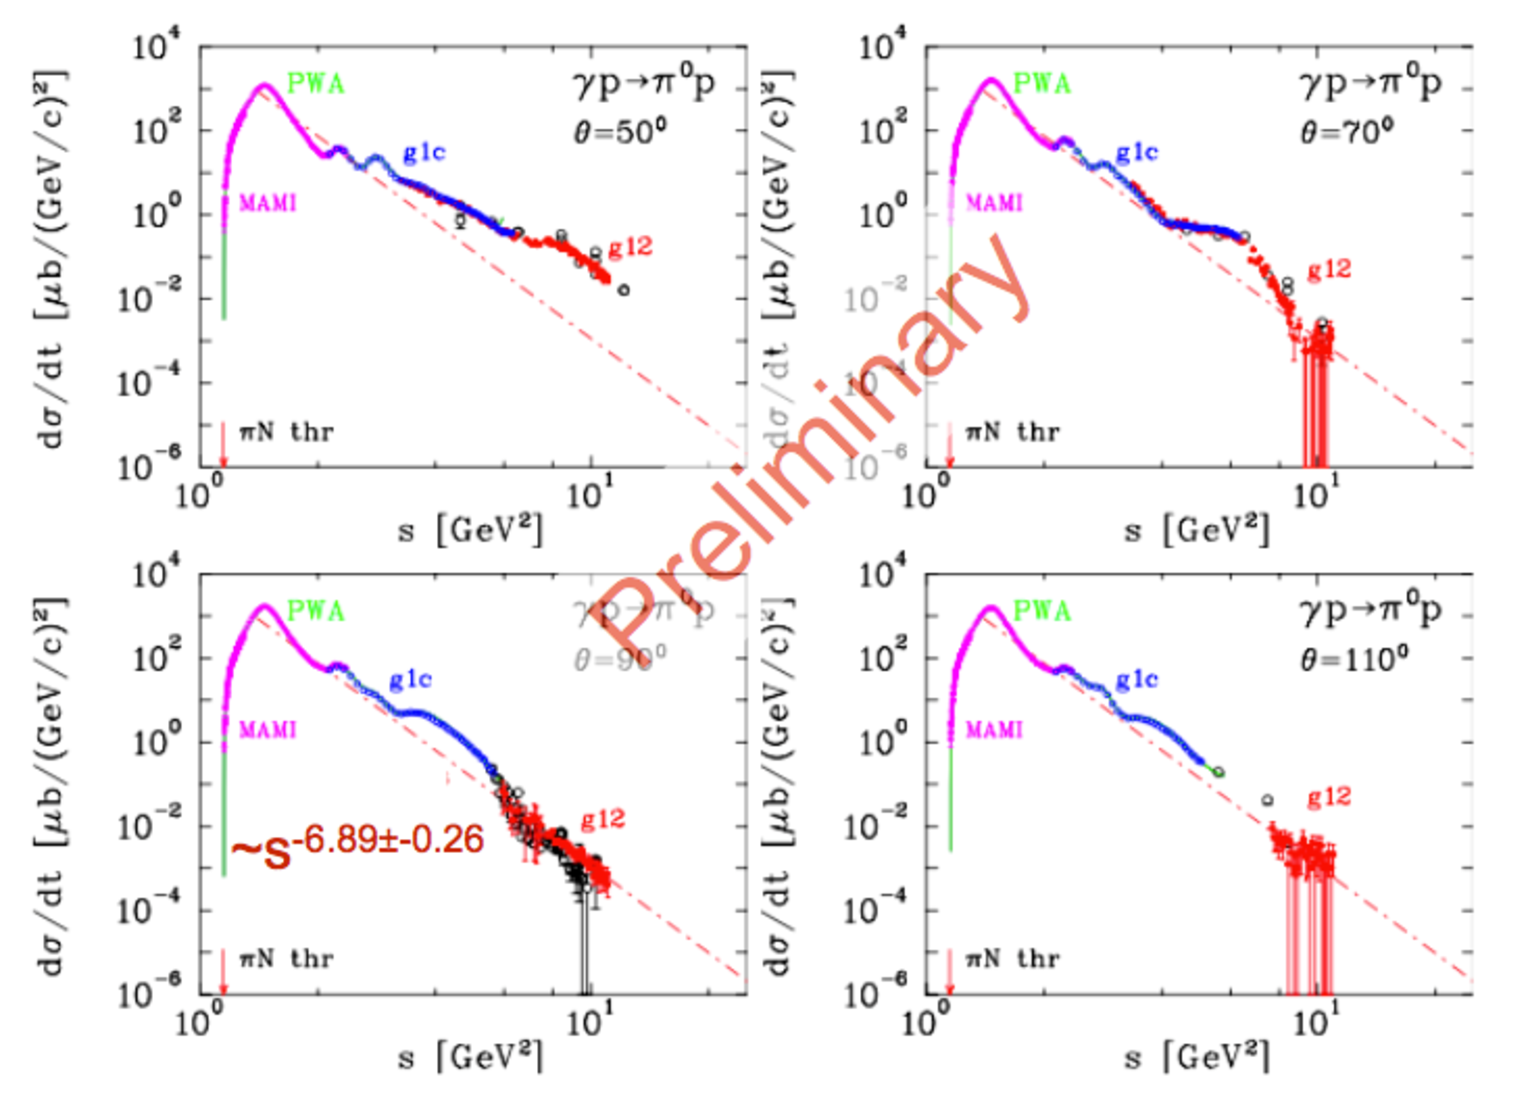
\includegraphics[width=250 pt]{figures/pi0_scaling.pdf}}
	\caption{Comparison with scaling rule. }
	\label{fig:pi0_scaling}
\end{figure}